\chapter{Quantum digital signatures}
Goal of chapter: introduce our QDS protocol and prove its security in different contexts using several methods.

\section{QDS protocol description}

In the simplest instance we may consider the signaure scheme involving only three parties: a sender, Alice ($A$), and recipients Bob ($B$) and Charlie ($C$). Alice wishes to send a classical message $m$ to $B$ and $C$, such that $B$ and $C$ can correctly determine whether $m$ was indeed sent by $A$. Furthermore the recipients should be able to check whether $m$ has been altered.

\subsection{Goals of a signature scheme}
\MT{Add introduction, and chat about how the multipartite setting is actually quite interesting}

A digital signature scheme must ensure that the following requirements are fulfilled:

\noindent \emph{$1$. Security against forgery}: Neither a dishonest recipient ($B$ or $C$), nor an external fourth party (Eve, $E$), should be able to alter $m$ and have it accepted as genuine by an honest recipient. That is, the signature scheme should ensure that $m$ is the message which Alice sent.

\noindent \emph{$2$. Genuine sender}: Neither a dishonest recipient ($B$ or $C$), nor an external fourth party (Eve, $E$), should be able to impersonate $A$. A message which falsely claims to have originated with Alice should be rejected.

\noindent \emph{$3$. Security against repudiation}: A dishonest sender $A$ should not be able to cause disagreement between $B$, $C$ about the previous two requirements. That is, after genuinely sending $m$ she should not later be able to deny it. If Bob accepts the message as genuine then so too should Charlie. 

\noindent \emph{$4$. Message transferability}: If $B$ accepts a message as genuine, then so too should $C$. In the simple $3$~party signatures protocol considered here, this requirement is equivalent to requirement $3$, while when more recipients are involved one may define a message $m^{\left(k\right)}$ as $k$-transferable if it can be successfully forwarded up to $k$ times. That is, if recipient $B_0$ accepts $m^{\left(k\right)}$, then recipients $B_1 \dots B_k$ should also accept.

For our scheme involving three parties (only two recipients), requirements $3$ and $4$ are equivalent, and so in what follows we will talk about repudiation only. Requirements $1$ and $2$ are fulfilled in our scheme by the same security process, and so we will focus on $1$ and simply note where $2$ arises.

\MT{Let's have a nice figure explaining each of these attacks, similar to the one from my CEWQO2018 poster, but without proprietary content}

A digital signature scheme which rejects all messages trivially fulfills requirements $1-4$, and so in order to get a useful digital signature scheme we impose:

\noindent \emph{$5$. Robustness}: In the absence of $E$, the message $m$ should be accepted if $A, B, C$ behave honestly.

\subsection{Our QDS scheme}

We here present a continuous-variable (CV) QDS protocol based on the quadrature phase-shift keying (QPSK) alphabet of coherent states. %this will be defined earlier, I am sure
Our protocol allows us to take into account quantum distribution channels which will in general be insecure, and this scheme is the first in the CV setting to be secure against eavesdropping. \MT{I should motivate the CV setting somewhere, probably in ch1}

Our QDS scheme is split into two stages, Distribution and Messaging, which can occur with significant time delay. The quantum states are sent and measured during Distribution, while during Messaging Alice will send her message and classical signature, and Bob and Charlie will try to determine its validity.\footnote{Note the intrinsic separation between the Distribution (quantum) and Messaging (classical) stages of the protocol. We will take further advantage of this separation between quantum and classical steps in Chapter~\MT{X}} Our protocol setup is outlined in Fig.~\MT{X}, while the protocol is described in Fig.~\MT{X} % I want a flowchart-style figure to outline the steps of the protocol

\MT{mention somewhere why we consider just a $1$ bit message}

\MT{I'll do everything for QPSK, but I should have a section where I generalize to NPSK}

\subsubsection{Distribution stage}
\noindent \underline{Step $1$.} Alice wishes to send a signed $1$ bit message $m$ to Bob and Charlie. For each possible future $m$, and for each recipient, Alice creates the following classical strings
\begin{equation}
\Phi_m^{\left(B, C\right)} = \left\{ \phi_{j, m}^{\left(B, C\right)}\right\}_{j=1}^{L}
\end{equation}
where the $\phi_{j}$ are complex phases chosen from alphabet $\mathcal{A}_4$. The $\phi_j$ are assumed to be drawn uniformly at random from $\mathcal{A}_4$, though we will relax this assumption in Chapter.~\MT{X}. The strings $\Phi_m^{\left(B, C\right)}$ are Alice's \emph{private key}. \MT{Talk somewhere about using a different private key for each recipient.} The signature length $L$ is an integer suitably chosen to ensure the desired level of security.
\par
\noindent \underline{Step $2$.} Corresponding to each of her private keys, Alice forms the following quantum states
\begin{equation}\label{eqn:QDS_publickey}
\rho\left[\Phi_m^{\left(B, C\right)}\right] := \otimes_{j=1}^L \rho\left[\phi_{j, m}^{\left(B, C\right)}\right]
\end{equation}
with
\begin{equation}
\rho\left[\phi_{j, m}^{\left(B, C\right)}\right] := \ket{\phi_{j, m}^{\left(B, C\right)}} \bra{\phi_{j, m}^{\left(B, C\right)}}
\end{equation}
understood to be the coherent state from $\mathcal{A}_4$ with phase corresponding to the relevant element of Alice's private key.

The states Eq.~\ref{eqn:QDS_publickey} may be interpreted simply as sequences of coherent states which Alice sends to each recipient. The states $\rho\left[\Phi_m^{\left(B, C\right)}\right]$ are Alice's \emph{public key}. \MT{talk somewhere about how the states she sends are different for each recipient.}
\par
\noindent \underline{Step $3$.} Each recipient $B, C$ performs heterodyne detection on each received $\rho\left[\phi_{j, m}^{\left(B, C\right)}\right]$ and receives complex phase outcome $x_{B,C}\in\mathbb{C}$. In other words, they perform the POVM
\begin{equation}
E\left[x\right] := \otimes_{j=1}^L E_j\left[x\right] \qq{with} E_j\left[x\right] := \frac{1}{\sqrt{\pi}} \ket{x}_j\bra{x}_j
\end{equation}
with $x \in \mathbb{C}$. Crucially, since measurement is performed immediately on receipt of the states, no quantum memory is required, and the remainder of the protocol is entirely classical.

At the end of the quantum stage of the protocol, recipients Bob and Charlie now each possess classical strings, length $L$, containing their complex phase measurements on Alice's distributed states, Fig.~\ref{fig:elimsig}~(a). They now form \emph{eliminated signatures}, Fig.~\ref{fig:elimsig}. For each complex outcome $x_j\in\mathbb{C}$, each recipient should record the phases $\phi_{j, m}^{\left(B, C\right)}$ which are \emph{least compatible} with $x_j$. For each element $j$, this may be understood as computing the four conditional probabilities 
\begin{equation}
p\left(\alpha_j | x_j\right) \qq{for each} \alpha_j \in \mathcal{A}_4,
\end{equation}
and recording the $\alpha_j$ giving rise to the smallest of these conditional probabilities. Note that these recorded $\alpha_j$ will always be adjacent elements of $\mathcal{A}_4$. An example of this elimination procedure is displayed pictorially in Fig.~\ref{fig:elimsig}, and for clarity we display the mapping explicitly in Tab.~\MT{X}. \MT{Create a table to illustrate the mapping to eliminated signatures.} We will denote Bob and Charlie's eliminated signatures at this stage as $X_m^{\left(B, C\right)}$. Each is of length $L$ and each will later be compared to Alice's public key in order to authenticate the message. 

\begin{figure}[htp]
\centering
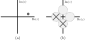
\includegraphics[width=0.8\linewidth]{qds/elimsig}
\caption{\label{fig:elimsig} \MT{(Draft)} (a) Bob and Charlie each perform heterodyne outcome on their received coherent states, and get complex outcome $x \in \mathbb{C}$. (b) They then record the two states from $\mathcal{A}_4$ which are least likely to have been sent by Alice.}
\end{figure}

\par
\noindent \underline{Step 4.} \emph{Symmetrization:} Bob and Charlie now swap a random $L/2$ elements of their $X_m^{\left(B, C\right)}$ over their secure classical channel. \MT{make sure I introduce this channel earlier}, and signature elements which have been forwarded by a player will no longer be used by him in the protocol. We denote these resulting strings as $Y_m^{\left(B, C\right)}$. Both the positions and the values of the swapped elements must be kept secret from Alice, which will ensure that the information which Bob and Charlie each hold is symmetric from Alice's point of view. 

In other words at the end of Step~$3$, having sent the state $\ket{\phi_{j, m}^B}\bra{\phi_{j, m}^B}$ to Bob, even though Alice does not know its value Alice knows that Bob holds the corresponding eliminated signature element $X_{j, m}^B$. At the end of Step~$4$ however, Alice does not know whether it is Bob or Charlie who holds $X_{j, m}^B$. This uncertainty will prove crucial for preventing her from successfully repudiating (Requirement~$3$). Bob and Charlie each now possess an eliminated signature $Y_m^{\left(B, C\right)}$ in two halves: one half containing those elements received directly from Alice, and one half containing elements received during this Symmetrization step.

\subsubsection{Messaging stage}





























